\documentclass[12pt]{report}
\usepackage{graphicx}
\usepackage{float}
\usepackage{lettrine}
\usepackage{caption}
\usepackage{url}
\usepackage[margin=1in]{geometry}
\usepackage{amsmath}
\usepackage{algorithm}
\usepackage[noend]{algpseudocode}
\usepackage{amssymb}

\newcommand\blfootnote[1]{%
  \begingroup
  \renewcommand\thefootnote{}\footnote{#1}%
  \addtocounter{footnote}{-1}%
  \endgroup
}

\title{Verification of GCD Circuits Using Algebraic Geometry}
\author{Jaden Simon - simonjaden223@gmail.com \\ \and
	   Daniel Humeniuk - d.humeniuk@utah.edu}

	   
\begin{document}

\maketitle

\section{Introduction}

The purpose of this report is to discuss our findings and results of our formal verification project for ECE 5745. Our original proposal was centered around verifying a 3-bit Elliptical Curve Arithmetic Unit (ECAU) circuit as a proof of concept. After some studying, our project led us to investigate the 3-bit greatest common divisor (GCD) circuit which would be required in finite field inversion. Our main point of investigation was to determine if verification of a 3-bit GCD circuit is trivial or nontrivial. Once this question could be answered, we could later explore if the verification could be easily transposed onto an $n$-bit GCD circuit.

This report will detail our findings as well as identified areas of further interest and exploration.

\section{Experiments and Test Setup}

Our first starting point was designing a circuit that computed a 3-bit GCD. This circuit can be seen in Figure \ref{fig:gcd}. Once this circuit was created, it took some refining to ensure that it would act as expected. 

\begin{figure}
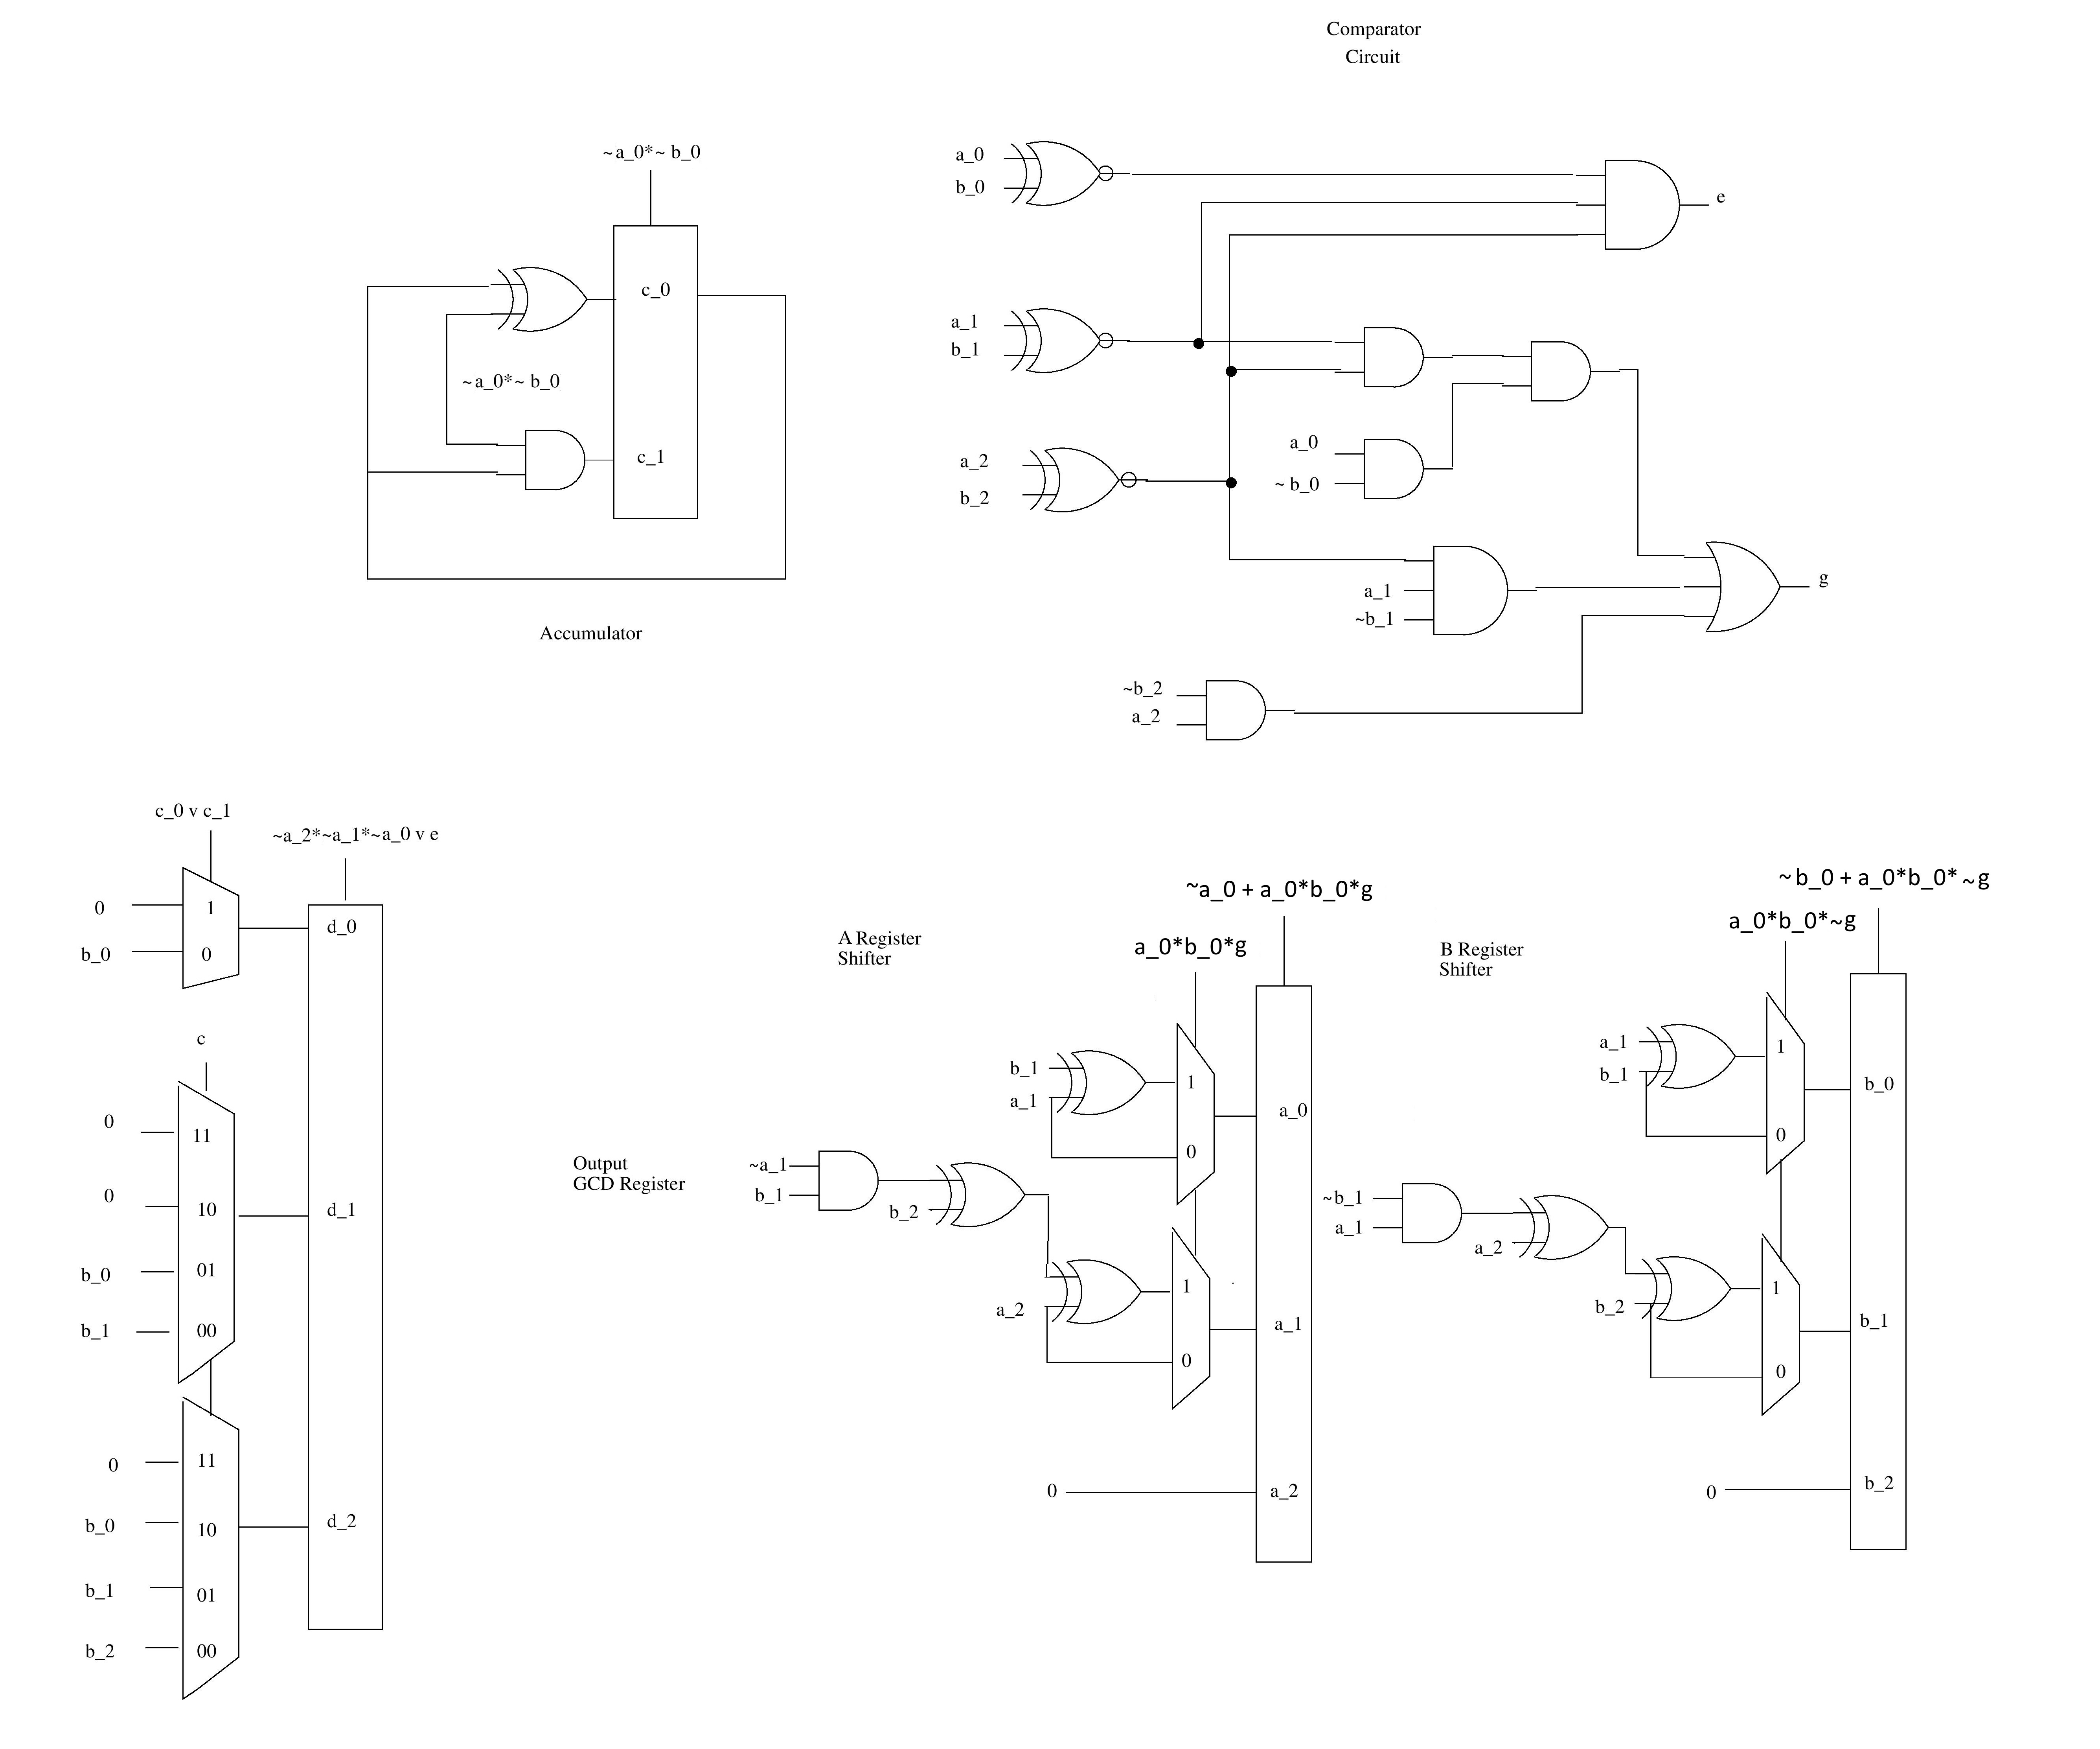
\includegraphics[scale=0.125]{images/gcd.png}
\caption{Binary GCD Algorithm for $3$ bits}
\label{fig:gcd}
\end{figure}

We first implemented the comparator circuit. This was mainly to see if we were doing things correctly. Mining the specification from this circuit was pretty ugly, so our expectations for the GCD circuit were rather low.

Then to test our knowledge of sequential circuits we made a simple variable 3-bit shifter, where the second input determines how many times the first should be shifted. This required the use of next state and present state variables. Registers were designed as muxs, where the register enable signal was the mux control signal. The next state value would then be the current state value if the enable signal was 0, otherwise it would be whatever was fed into it if it was 1. This worked well and we were able to simulate operations. 

The GCD circuit was built using the same strategy as above, where registers were just muxs. Even for just a simple 3-bit circuit, there were over 40 polynomials that described it. Automating the generation of arbitrary GCD circuits would be necessary for further experimentation. Writing these kinds of circuits by hand is incredibly tedious, especially when it comes to debugging. 

We were unable to get the circuit to work over the field $\mathbb{Q}$. There were issues that are far too tedious to fix for such a short time frame. Automation scripts would be very helpful here, allowing the easy conversion of a circuit over different fields.

\section{Findings}

Our first finding was very interesting. When we were performing the verification, we were conducting the experiment over a finite field. This resulted in our discovery verification for this particular circuit would not work over a finite field as every element within a finite field divides every other element. Our circuit could have been simplified to returning either A or B as either one divides the other. To make an integer version of our circuit, we simply needed to add a few gates to perform integer subtraction. 

With the GCD circuit, we were able to get a specification polynomial in terms of two inputs $A$ and $B$ (Figure \ref{fig:spec}), however, this polynomial is very ugly looking and does not tell us much. Note that in this case $C$ can be set to 0 as part of a reset state and $n\_C$ can be composed of $A$ and $B$. We imagine that higher $n$-bit circuits would create worse looking specifications. Since the gate-level variables are often unnecessary when it comes to verification, we used projection of varieties to get rid of all gate-level variables in our outputs.

\begin{figure}
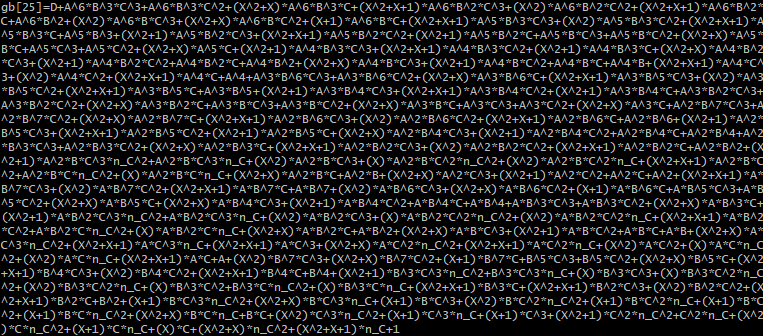
\includegraphics[scale=0.5]{images/ff_gcd_output.png}
\caption{Specification of 3-bit GCD circuit}
\label{fig:spec}
\end{figure}

Another interesting thing we found is that using word-level polynomials over $\mathbb{Q}$ caused some of the polynomials to explode. Our comparator circuit was converted and tested, with our results looking like Figure \ref{fig:boom}. This specification seems very random and would not be much use to us. We think that the GCD circuit would output something similar to this if we used word-level variables. 

\begin{figure}
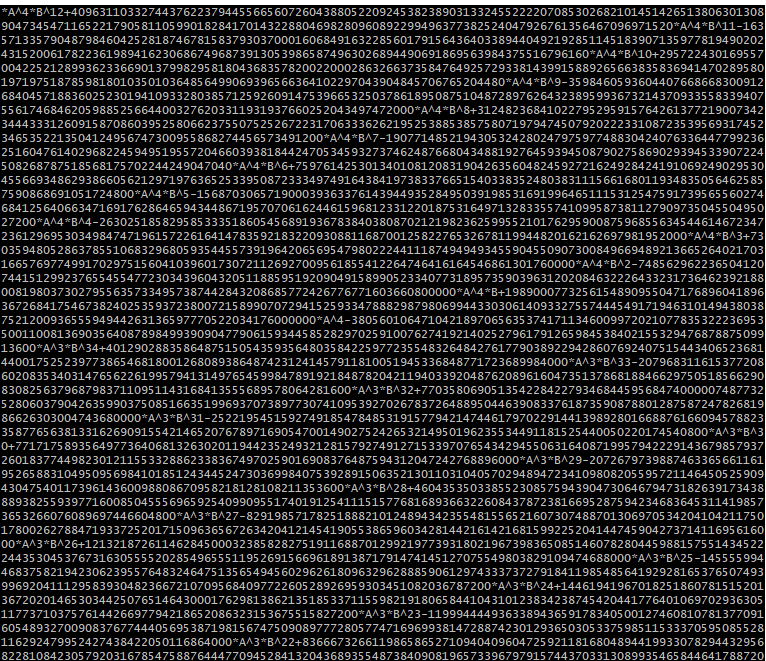
\includegraphics[scale=0.5]{images/q_comp_output.png}
\caption{Part of the output from the comparator circuit over rational numbers}
\label{fig:boom}
\end{figure}

\section{Conclusion}

The verification of the GCD circuit proved to be a very interesting project to work on. More research will need to be conducted to determine the exact nature of the problem. There also remains the question of the use of a GCD circuit in real world applications. Finite field arithmetic in hardware has many options in regards to finding an element's inverse, extended GCD is one option but there are other, faster ways. Seeing the specification polynomial over $\mathbb{Q}$ would have been interesting, but unfortunately we just ran out of time. Verifying these circuits is hard.

\bibliographystyle{IEEEtran}

%\bibliography{IEEEabrv,bib/ref}

\end{document}